% fig04_mhd_thrust — Stage-2 cruise per-channel F_MHD = J*B*V across altitude.
% Standalone pgfplots; compiled to figures/fig04_mhd_thrust.pdf.
% Comparison (thrust vs altitude) => chart (commons comparison rule).
% Data: Appendix B, UFO/verify/stage2-cruise-mhd.md (triple_product anchors).
%   20 km : J=2.0e5 B=5 V=0.096 -> 96000 N
%   100 km: J=1.5e5 B=4 V=0.096 -> 57600 N
%   200 km: J=1.0e5 B=3 V=0.096 -> 28800 N
%   craft weight mg = 650*9.81 = 6376.5 N
\documentclass[border=4pt]{standalone}
\usepackage{tikz}
\usepackage{pgfplots}
\pgfplotsset{compat=1.18}
\begin{document}
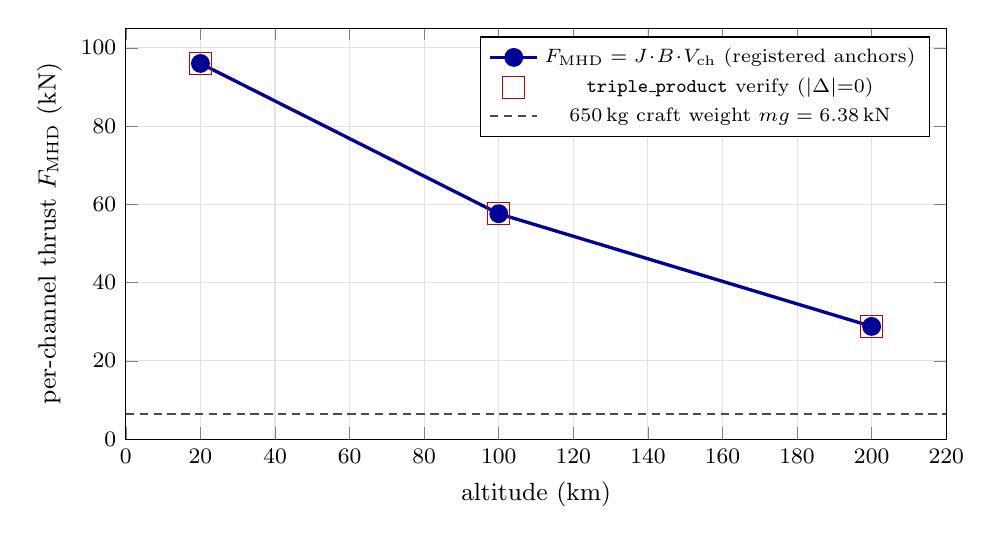
\begin{tikzpicture}
\begin{axis}[
  width=12cm, height=6.8cm,
  xlabel={altitude (km)},
  ylabel={per-channel thrust $F_{\mathrm{MHD}}$ (kN)},
  xmin=0, xmax=220, ymin=0, ymax=105,
  tick label style={font=\footnotesize},
  label style={font=\small},
  ymajorgrids, xmajorgrids, grid style={gray!22},
  legend style={font=\scriptsize, at={(0.98,0.98)}, anchor=north east},
]
\addplot[blue!60!black, very thick, mark=*, mark size=2.8pt] coordinates {
  (20, 96.0) (100, 57.6) (200, 28.8)
};
\addlegendentry{$F_{\mathrm{MHD}}=J\!\cdot\!B\!\cdot\!V_{\mathrm{ch}}$ (registered anchors)}
\addplot[only marks, mark=square, mark size=4pt, red!75!black] coordinates {
  (20, 96.0) (100, 57.6) (200, 28.8)
};
\addlegendentry{\texttt{triple\_product} verify ($|\Delta|{=}0$)}
\addplot[gray!60!black, thick, densely dashed, domain=0:220] {6.3765};
\addlegendentry{650\,kg craft weight $mg=6.38$\,kN}
\end{axis}
\end{tikzpicture}
\end{document}
